\documentclass{article}
\usepackage{tikz}
\usetikzlibrary{angles, quotes}
\usepackage{amssymb}
\usepackage{physics}
\usepackage{pgfplots}
\pgfplotsset{width=10cm,compat=1.9}
\usepgfplotslibrary{statistics}
\usepackage[left=2.54cm,right=2.54cm,top=2.54cm,bottom=2.54cm]{geometry}
\usepackage{tasks} %Paquete necesario para la producción de items horizontales para algunos ejercicios de tarea empleando el comando /begin{multicols}}{#}.../end{multicols} para ayudarnos a reducir las páginas
\usepackage{pdflscape} %comando que permite cambiar a orientación horizontal las hojas%
\usepackage{soul} %Paquete para permitir la compilación de acentos usando el comando {\hl{}}}\\
\sethlcolor{yellow(munsell)} %comando para definir el color para el subrayado usando el comando \hl
\usepackage[utf8]{inputenc}
\usepackage[spanish]{babel}
\usepackage{icomma}
\usepackage{ragged2e}		
\usepackage{siunitx}
\usepackage{url}
\usepackage[colorlinks=true, urlcolor=blue,  linkcolor=Cerulean, citecolor=green]{hyperref}
\usepackage{pdfpages}
\usepackage{blindtext} %Paquete que genera texto ficticio (dummy text) con el comando: \blindtext
\usepackage{cancel} %in the preamble gives you four different modes of striking through: \cancel{text to cancel} draws a diagonal line (slash) through its argument, \bcancel{text to cancel} uses the negative slope (a backslash), \xcancel{text to cancel} draws an X (actually \cancel plus \bcancel), \cancelto{〈value〉}{〈expression〉} draws a diagonal arrow through the 〈expression〉pointing to the 〈value〉 (math-mode only)
\usepackage{csquotes}
\usepackage{afterpage}
\usepackage{parskip} 
\usepackage{float}
\usepackage{enumitem}
%\usepackage{multicol}%Paquete que permite la creación aislada de columnas de texto. De esta forma se reduce la cantidad de páginas en nuestro documento
\usepackage{lipsum} %Paquete que genera texto de relleno al igual que \usepackage{blindtext}, se usa con el comando \lipsum[#-#] los #(hashtags) delimitan el número de páginas que deseamos ocupar del paquete lipsum para usarlos como relleno. 

% Definir el comando personalizado para la nota
\newcommand{\mynote}[1]{%
\begin{tikzpicture}[baseline=-0.75ex]
\node[draw, circle, fill=Apple Green!60, inner sep=2pt] (note) {\textbf{Nota:}};
\end{tikzpicture}%
\ \textit{#1}%
}

% Definición de comandos para variables con barra
\newcommand{\xbar}{\overline{x}}
\newcommand{\ybar}{\overline{y}}

\newenvironment{Figura}
{\par\medskip\noindent\minipage{\linewidth}}
{\endminipage\par\medskip}
\usepackage{caption}
\usepackage[
backend=biber,
sorting=none,
url=true
]{biblatex} %bibliografía
\addbibresource{biblio.bib}
% Establecer el espacio entre las entradas de la bibliografía
\setlength{\bibitemsep}{1\baselineskip} % Puedes ajustar el valor según tus preferencias
\usepackage{amsmath,amsthm,amssymb,amsfonts}
\usepackage{pifont} %Permite la compilación del comando \xmark: es el símbolo de la tachita
\usepackage{mathtools} %permite la compilación de símbolos para matrices
\usepackage{empheq} %Paquete que se relaciona con \usepackage[most]{tcolorbox} para la creación de cuadros/cajas de colores para delimitar los resultados matemáticos o líneas de texto usando la línea de comando: \begin{empheq}[box={\mymath[colback=orange(webcolor)!70,drop lifted shadow]}]{equation*} \end{empheq}
\usepackage[most]{tcolorbox} %Paquete que se relaciona con \usepackage{empheq} para la creación de cuadros/cajas de colores para delimitar los resultados matemáticos o líneas de texto
\renewcommand{\qedsymbol}{$\blacksquare$}
\usetikzlibrary{positioning,decorations.pathreplacing} %Paquete que permite la compilación de llaves para cuadros sinópticos (brace diagram) 
\usepackage{schemata} %The schemata package is designed just for these brace diagrams
\usepackage{booktabs}

\newcommand\AB[2]{\schema{\schemabox{#1}}{\schemabox{#2}}} %comando o paquete necesario para crear cuadros sinópticos

\newtcbox{\mymath}[1][]{%
nobeforeafter, math upper, tcbox raise base,
enhanced, colframe=blue!30!black,
colback=blue!30, boxrule=1pt,
#1} %Comando importante para encasillar los resultados matemáticos en cajas de diferentes colores, se relaciona con los paquetes \usepackage{empheq} y \usepackage[most]{tcolorbox} 

\newenvironment{sysmatrix}[1]
{\left(\begin{array}{@{}#1@{}}}
{\end{array}\right)}
\newcommand{\ro}[1]{%
\xrightarrow{\mathmakebox[\rowidth]{#1}}%
}
\newlength{\rowidth}% row operation width
\AtBeginDocument{\setlength{\rowidth}{3em}}  %Comando importante para laproducción de lineas de operaciones entre matrices, método de Gauss o Gauss Jordan se relaciona con \newenvironment{sysmatrix}

%formato para cambiar el horario a español
\usepackage[spanish]{datetime2}
\DTMsetdatestyle{spanish}

\renewcommand{\today}{\DTMdisplaydate{\the\year}{\the\month}{\the\day }{-1}}
%%%%%%%%%%%%%%%%%%%%%%%%%%%%%%%%%%%%%%%%%

\usepackage{datetime}
\newcommand{\mycurrenttime}{\xxivtime}

%%%%%%%%%%%%%%%%%%%%%%%%%%%%%%%%%%%%%%%%%%%%%%%%%%%%%%%%%%%%%%%%%%%%%%%%%%%%%%%%%%%%%%%%%%%%%%%%%%%%%%%%%%%%%%%%%%%%%%%%%%%%%%%%%%%%%%%%%%%%%%%%%


%%%%%%%%%%%%%Caja de color para el título%%%%%%%%%%%%%%%%%%%%%%%%%%%%%%%%%%%%%%%%%%%%%%%%%%%%%%

\definecolor{myframecolor}{RGB}{1, 45, 75} % Prussian Blue
\definecolor{myboxcolor}{RGB}{0, 107, 92} % Apple Green

\newtcolorbox{mybox}{
enhanced,
colback=myboxcolor!7, % Color de fondo del cuadro
colframe=myframecolor, % Color del marco del cuadro
arc=0pt,
boxrule=1pt,
borderline west={2mm}{-10mm}{myframecolor}, % Borde en el lado izquierdo
sharp corners=southwest,
width=\linewidth,
before=\par\vspace{\bigskipamount}, % Espacio antes del cuadro
after=\par\vspace{\bigskipamount} % Espacio después del cuadro
}

%%%%%%%%%%%%%%%%%%%%%%%%%%%%%%%%%%%%%%%%%%%%%%%%%%%%%%%%%Nueva caja%%%%%%%%%%%%%%%%%%%%%%%%%%%%%%%%%%%%%%%%%%%%%%%%%%%%%%%%%%%%%%%%%

\newtcolorbox{mybox2}{
enhanced,
colback=Apple Green!7, % Color de fondo del cuadro
colframe=Apple Green, % Color del marco del cuadro
arc=0pt,
boxrule=1pt,
borderline west={2mm}{-10mm}{Apple Green}, % Borde en el lado izquierdo
sharp corners=southwest,
width=\linewidth,
before=\par\vspace{\bigskipamount}, % Espacio antes del cuadro
after=\par\vspace{\bigskipamount} % Espacio después del cuadro
}


\newcommand{\euler}{e} %Comando para producir letra e de euler
\newenvironment{remark}{\par\vfill\footnotesize % Vertical white space above the remark and smaller font size
\begin{list}{}{
	\leftmargin=80pt % Indentation on the left
	\rightmargin=60pt}\item\ignorespaces % Indentation on the right
\makebox[-2.5pt]{\begin{tikzpicture}[overlay]
		\node[draw=Horizon!60,line width=2.5pt,circle,fill=Horizon!25,font=\sffamily\bfseries,inner sep=4pt,outer sep=0pt] at (-19pt,5pt){\textcolor{Horizon}{Nota}};\end{tikzpicture}} % Blue Nota in a circle
\advance\baselineskip -1pt}{\end{list}\vskip5pt} % Tighter line spacing and white space after remark
\usepackage{graphicx}

\usepackage{titling}

\input{colores.tex}

%%Producir signos de cita textual``Asignatura''

\newcommand{\xmark}{\ding{55}} %%%comando que genera la tachita

\newenvironment{MyColorPar}[1]{%
\leavevmode\color{#1}\ignorespaces%
}{%
}%

%%%%%%%%%%%%%%%%%%% Título de la tarea, Nombre de alumno

\title{ \textcolor{Sun}{\textbf{Kepler: recuperación}}}
\author{\emph{Julio Alfredo Ballinas García} $\boldsymbol{\mid}$ \textcolor{Tarawera}{\textbf{202107583}}}
\date{\today}

%%%%%%%%%%%%%%%%%%% Datos de la Materia

\usepackage{fancyhdr}
\fancypagestyle{plain}{%  the preset of fancyhdr 
\fancyhf{} % clear all header and footer fields
\fancyfoot[R]{
\includegraphics[width=2cm]{LogoFCFMBUAP (1).png}}
\fancyfoot[L]{{\bfseries{\thedate{}}} a las {\bfseries{\mycurrenttime{}}} horas{} (GMT-6, H. Puebla de Zaragoza, Pue)}
\fancyhead[L]{\textbf{Asignatura:} Mecánica teórica}
\fancyhead[R]{\theauthor}
}
\makeatletter
\def\@maketitle{%
\newpage
\null%
\begin{center}%
\let \footnote \thanks
{\LARGE \@title \par}%
\vskip 1em%
%{\large \@date}%
\end{center}%
}
\makeatother

\usepackage{lipsum}  
\usepackage{cmbright}


%%%%%%%%%%%%%%%%%%%%%%%%%%%%%%%%%%%%%%%%%%%%%%%%%%%%%%%%%%%%%%%%%%%%%%%%%%%%%%%%%%%%%%%%%%%%%%%%%%%%%%%%%%%%%%%%%%%%%%%%%%%%%%%%%%%%%%%%%%%%%%%%%%%%%%%%%%%%%%%%%%%%%%%%%%%%%%%%%%%%%%%%%%%%%%%%%%%%%%

% Por si el color se llama "Apple Green" con espacio en colores.tex:
\colorlet{AppleGreen}{Apple Green}

% Caja AppleGreen con tono ajustable
\newenvironment{AGbox}[1][7]% 7 = tono por defecto (más grande => más claro)
{%
  \begin{tcolorbox}[
    enhanced, breakable,
    colframe=AppleGreen,
    colback=AppleGreen!#1,
    boxrule=1pt,
    borderline west={2mm}{-10mm}{AppleGreen},
    sharp corners=southwest,
    left=14pt,right=14pt,top=10pt,bottom=10pt,
     boxsep=6pt,
  ]%
}{%
  \end{tcolorbox}%
}


\begin{document}



\maketitle

%%%%%%%%%%%%%%%%%%% Datos del profesor, campus, aula e integrantes

\begin{mybox2}
\noindent
\begin{tabular}{@{}p{3.7cm}p{10.4cm}@{}}
\textbf{Profesor} & Dr. Gilberto Silva Ortigoza \\[3pt]
\textbf{Campus / Facultad} & \textcolor{prussianblue}{\textbf{C.U. BUAP}} / \textcolor{trueblue}{\textbf{FCFM}} \\[3pt]
\textbf{Edificio / Salón} & \textcolor{prussianblue}{\textbf{EMA4}} / \textcolor{trueblue}{\textbf{302}} \\[6pt]
\end{tabular}
\end{mybox2}
\vspace{1cm}


% Solo el índice en negro y en negritas
\hypersetup{linkcolor=black}   % (opcional: urlcolor=black, citecolor=black)
{\bfseries \tableofcontents}
\hypersetup{linkcolor=Cerulean} % regresamos a tu paleta

\vspace{0.5cm}
\begin{center}
\begin{tikzpicture}
	% Dibuja círculos rellenos en diferentes colores
	\fill[bittersweet] (0,0) circle (0.17cm);
	\fill[Apple Green] (0.6,0) circle (0.17cm);
	\fill[trueblue] (1.2,0) circle (0.17cm);
	\fill[Aguamarina] (1.8,0) circle (0.17cm);
	\fill[Sun] (2.4,0) circle (0.17cm);
	\fill[orange(colorwheel)] (3.0,0) circle (0.17cm);
	\fill[Pesto] (3.6,0) circle (0.17cm);
	\fill[blue-violet] (4.2,0) circle (0.17cm);
	\fill[ticklemepink] (4.8,0) circle (0.17cm);
	\fill[Gallery] (5.4,0) circle (0.17cm);
	\fill[Mantle] (6.0,0) circle (0.17cm);
	\fill[Nevada] (6.6,0) circle (0.17cm);
	\fill[onyx] (7.2,0) circle (0.17cm);
	% Agrega más círculos o modifica los colores según sea necesario
\end{tikzpicture}
\end{center}  \vspace{0.5cm}

\setlength{\columnsep}{2cm}
\section*{\textcolor{Tarawera}{\textbf{Kepler: recuperación}}}
\addcontentsline{toc}{section}{Problemas: \textcolor{Tarawera}{\textbf{Kepler: recuperación}}}


%=========================================================
%                      Problema 1
%=========================================================

\addcontentsline{toc}{subsection}{\textcolor{Apple Green}{\textbf{\underline{Problema 1}}}}
\begin{AGbox}[8]
\textcolor{Apple Green}{\textbf{\underline{Problema 1}}} \vspace{2mm}

Escriba correctamente las leyes de Kepler. \hfill [3 puntos]

\end{AGbox}
\vspace{0.5cm}

\textcolor{Tuscany}{\textbf{Solución:}}

En este problema se nos pide enunciar de manera clara y \emph{correcta} las tres
\textcolor{Tarawera}{\textbf{leyes de Kepler}} para el movimiento de los planetas alrededor del Sol.  
Estas leyes describen el movimiento orbital suponiendo que:

\begin{itemize}
  \item[$\bullet$] Los planetas se mueven bajo la acción gravitacional dominante del Sol
  \item[$\bullet$] La interacción entre planetas se desprecia (aproximación de \emph{dos cuerpos})
\end{itemize}

A continuación, presentamos cada ley con su nombre tradicional, una redacción
clara y su contenido \textbf{matemático esencial}, conectándolas con la formulación
newtoniana del \emph{problema de Kepler}.

\vspace{0.4cm}

%---------------------------------------------------------
% 1) Primera ley de Kepler
%---------------------------------------------------------
\noindent
\textcolor{Apple Green}{\textbf{\underline{Primera ley de Kepler (ley de las órbitas)}}}

\begin{itemize}
  \item[$\bullet$]
  Cada planeta se mueve alrededor del Sol en una \textcolor{Lochinvar}{\textbf{órbita elíptica}},
  con el \textcolor{Cinnabar}{\textbf{Sol ubicado en uno de los focos}} de la elipse.
\end{itemize}

Geométricamente, esto significa que la trayectoria del planeta no es un círculo
perfecto, sino una \underline{elipse} caracterizada por su \emph{semieje mayor} \(a\),
\emph{semieje menor} \(b\) y \emph{excentricidad} \(e\), con
\begin{equation}
\begin{split}
e &= \sqrt{1 - \frac{b^{2}}{a^{2}}}
\end{split}\label{eq:def_excentricidad}
\end{equation}

Tomando coordenadas polares \((r,\theta)\) con origen en el foco ocupado por el Sol,
la órbita se escribe como una \textcolor{trueblue}{\textbf{cónica}} con parámetro focal \(p\):
\begin{equation}
\begin{split}
r(\theta)
&= \frac{p}{1 + e\cos\theta}
\end{split}\label{eq:orbita_eliptica}
\end{equation}
donde, para el problema de Kepler con fuerza central gravitacional
\(\displaystyle F(r) = -\frac{GMm}{r^{2}}\), el parámetro focal está dado por
\begin{equation}
\begin{split}
p &= \frac{\ell^{2}}{GMm^{2}}
\end{split}\label{eq:parametro_focal}
\end{equation}
y \(\ell\) es el \textcolor{vividviolet}{\textbf{momento angular}} del planeta respecto al Sol.

\vspace{0.4cm}

%---------------------------------------------------------
% 2) Segunda ley de Kepler
%---------------------------------------------------------
\noindent
\textcolor{vividviolet}{\textbf{\underline{Segunda ley de Kepler (ley de las áreas)}}}

\begin{itemize}
  \item[$\bullet$]
  El radio vector que une el \textcolor{Tarawera}{\textbf{planeta}} con el
  \textcolor{orange(colorwheel)}{\textbf{Sol}} barre \emph{áreas iguales en tiempos iguales}
\end{itemize}

Sea \(\vec r(t)\) la posición del planeta medida desde el Sol y \(A(t)\) el área
barrrida por el radio vector en el intervalo de tiempo considerado. La segunda ley
se expresa de manera compacta como
\begin{equation}
\boxed{
\frac{\dd A}{\dd t} = \text{constante}
}
\label{eq:segunda_ley_kepler}
\end{equation}

En coordenadas polares, el área barrida por el radio vector satisface
\begin{equation}
\begin{split}
\frac{\dd A}{\dd t}
&= \frac{1}{2}\,r^{2}\,\dot\theta
\end{split}\label{eq:areal_velocity}
\end{equation}
pero, para una \textcolor{Tarawera}{\textbf{fuerza central}} (como la gravedad newtoniana),
el momento angular \(\ell\) se conserva:
\begin{equation}
\begin{split}
\ell
&= m r^{2}\dot\theta
= \text{constante}
\end{split}\label{eq:momentum_angular_const}
\end{equation}
Sustituyendo \eqref{eq:momentum_angular_const} en \eqref{eq:areal_velocity}, se obtiene
\begin{equation}
\boxed{
\frac{\dd A}{\dd t}
= \frac{\ell}{2m}
= \text{constante}
}
\label{eq:areal_velocity_const}
\end{equation}
que es la forma \textcolor{Lochinvar}{\textbf{dinámica}} de la segunda ley de Kepler: el barrido de áreas
es constante porque el momento angular se conserva.

Esto implica que el movimiento es \textcolor{trueblue}{\textbf{no uniforme}} en términos de la velocidad
angular: el planeta se mueve más rápido cuando está cerca del Sol (\emph{perihelio})
y más lento cuando está lejos (\emph{afelio}), de modo que el \emph{barrido de áreas}
por unidad de tiempo se mantiene constante.

\vspace{0.4cm}

%---------------------------------------------------------
% 3) Tercera ley de Kepler
%---------------------------------------------------------
\noindent
\textcolor{Lochinvar}{\textbf{\underline{Tercera ley de Kepler (ley de los períodos)}}}

\begin{itemize}
  \item[$\bullet$]
  El \textcolor{Cinnabar}{\textbf{cuadrado del período}} orbital \(T\) de un planeta es
  proporcional al \textcolor{Apple Green}{\textbf{cubo del semieje mayor}} \(a\) de su órbita elíptica
\end{itemize}

En forma matemática, para un planeta que orbita al Sol se tiene
\begin{equation}
\boxed{
T^{2} \propto a^{3}
}
\label{eq:tercera_ley_proporcional}
\end{equation}
En la formulación newtoniana del problema de Kepler, para una masa central \(M\)
y constante gravitacional \(G\), la relación se vuelve \emph{exacta}:
\begin{equation}
\boxed{
T^{2}
= \frac{4\pi^{2}}{GM}\,a^{3}
}
\label{eq:tercera_ley_newtoniana}
\end{equation}
Es decir,
\begin{equation}
\begin{split}
K
&= \frac{4\pi^{2}}{GM}
\end{split}\label{eq:K_def}
\end{equation}
en la notación
\(\displaystyle T^{2} = K a^{3}\).  
Para todos los planetas que orbitan la misma masa central \(M\) (el Sol), la razón
\(\displaystyle T^{2}/a^{3}\) es la \emph{misma constante}:
\begin{equation}
\boxed{
\frac{T^{2}}{a^{3}}
= \frac{4\pi^{2}}{GM}
= \text{constante para todos los planetas que orbitan al Sol}
}
\label{eq:tercera_ley_constante}
\end{equation}

\vspace{0.4cm}

En resumen, las tres leyes de Kepler:

\begin{itemize}
  \item[$\bullet$] Describen la \textcolor{Tarawera}{\textbf{forma geométrica}} de las órbitas
        mediante la ecuación elíptica \eqref{eq:orbita_eliptica}
  \item[$\bullet$] Fijan la \textcolor{vividviolet}{\textbf{ley de barrido de áreas}}
        a través de la constancia de \(\ell\) en \eqref{eq:areal_velocity_const}
  \item[$\bullet$] Relacionan el \textcolor{Apple Green}{\textbf{período orbital}} y el
        \textcolor{orange(colorwheel)}{\textbf{tamaño de la órbita}}
        mediante \eqref{eq:tercera_ley_newtoniana}
\end{itemize}

y constituyen la base fenomenológica y matemática del
\textcolor{trueblue}{\textbf{problema de Kepler}} en mecánica celeste clásica.

\begin{figure}[H]
  \centering
  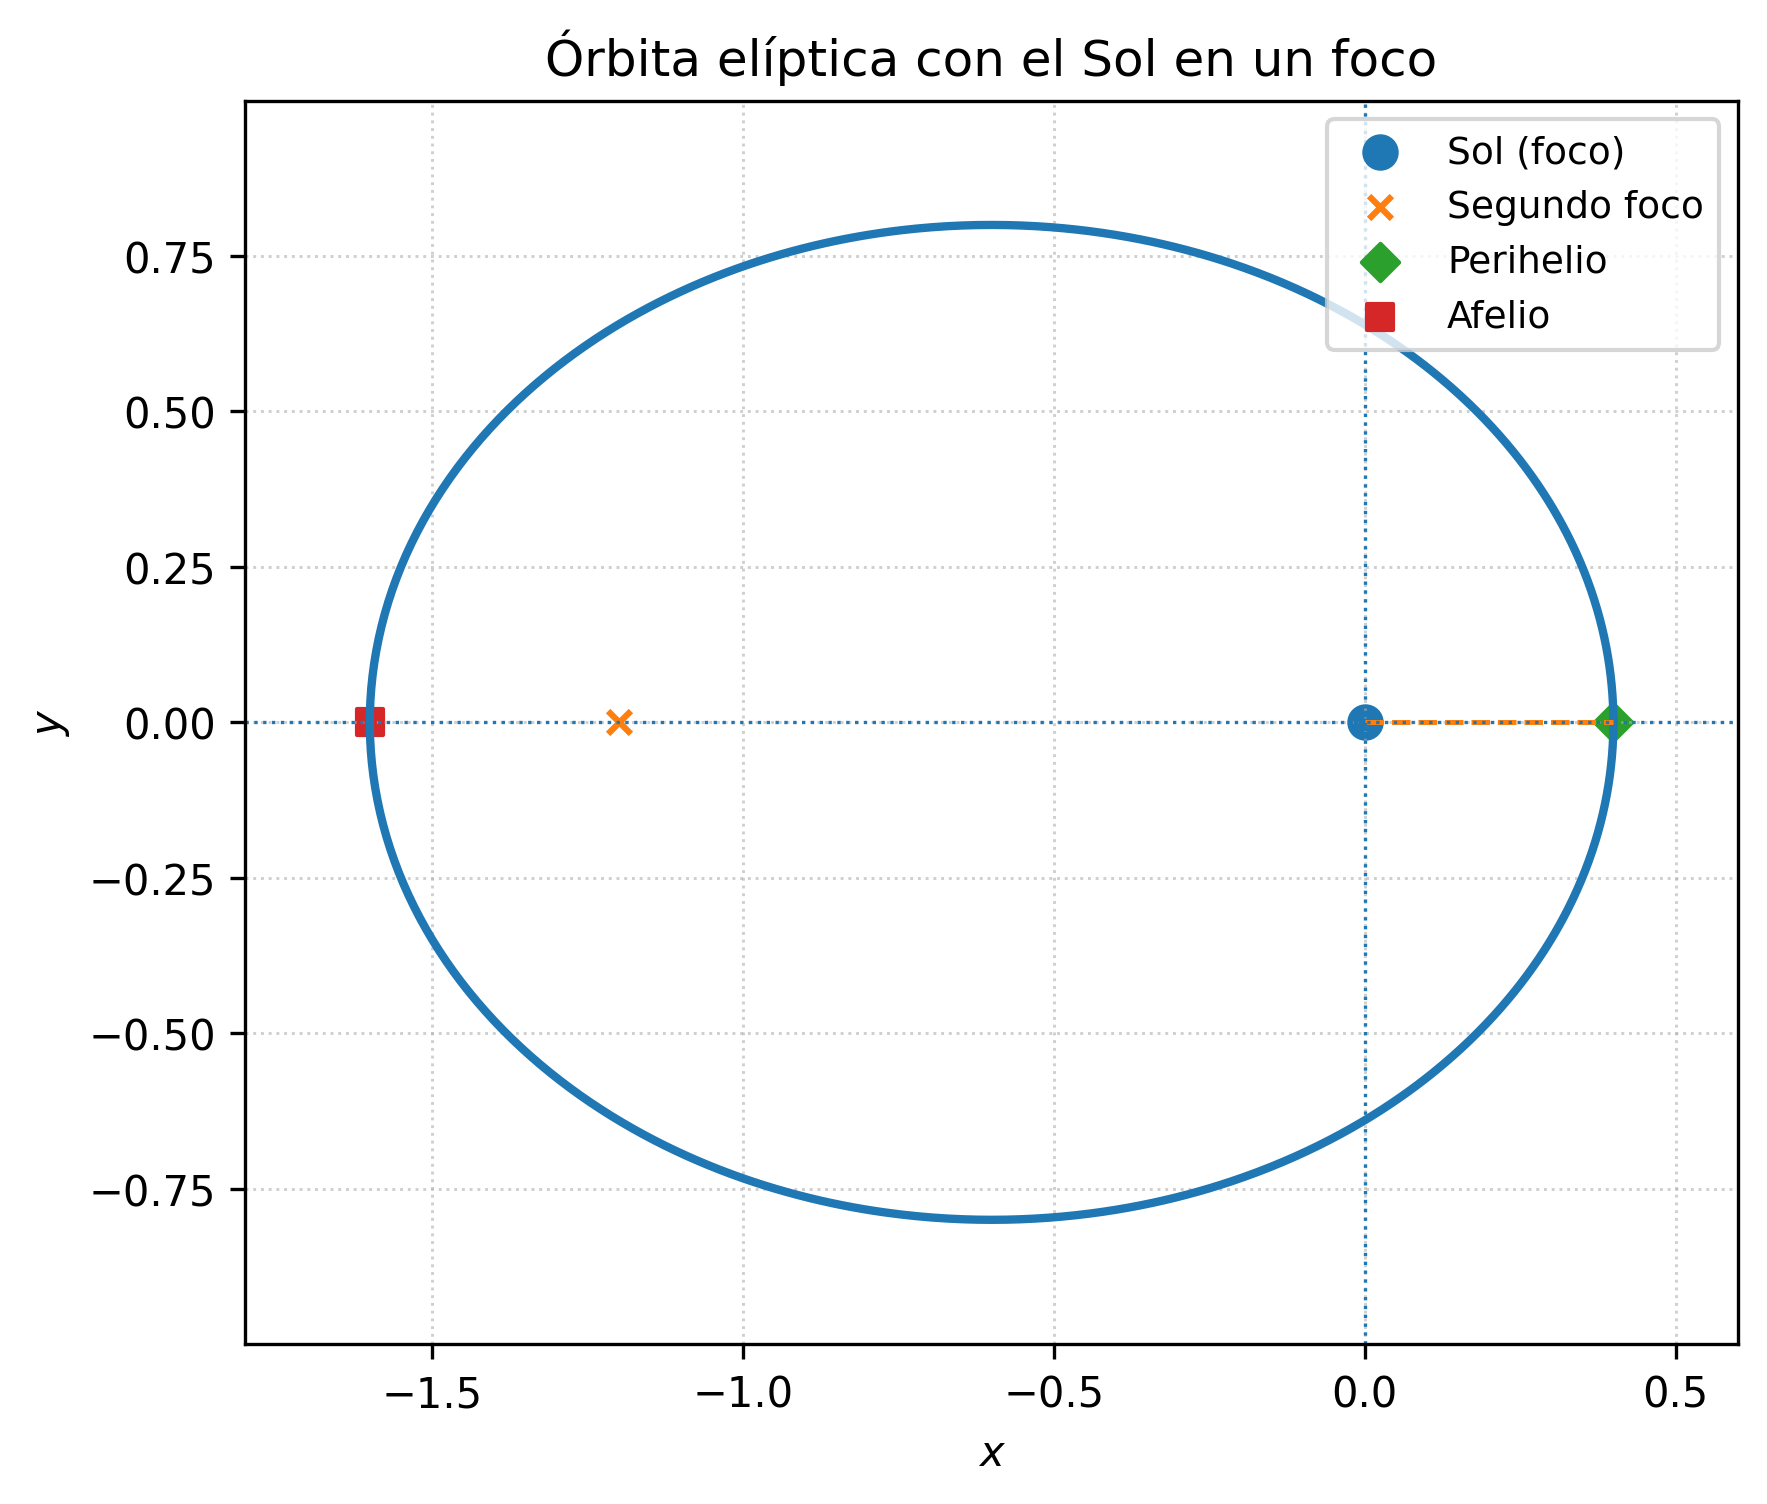
\includegraphics[width=0.6\textwidth]{kepler_orbita_eliptica.png}
  \caption{Representación de una órbita elíptica con el Sol en uno de los focos,
  mostrando el perihelio, el afelio y los dos focos de la elipse.}
  \label{fig:kepler_orbita_eliptica}
\end{figure}

\begin{figure}[H]
  \centering
  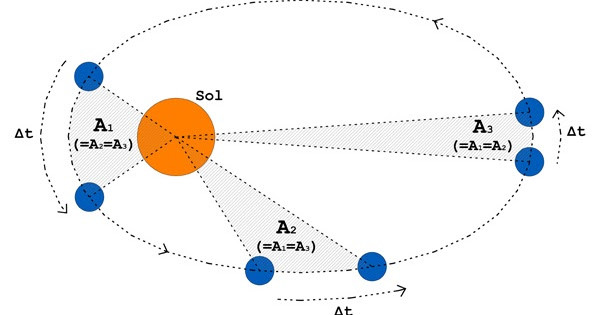
\includegraphics[width=0.7\textwidth]{KEPLER_2.jpg}
  \caption{Ilustración de la segunda ley de Kepler. El radio vector que une
  el Sol con el planeta barre áreas iguales en tiempos iguales: las dos
  regiones sombreadas tienen, dentro de la aproximación numérica, el mismo
  área aunque correspondan a distintos tramos de la órbita.}
  \label{fig:kepler_segunda_ley}
\end{figure}





%=========================================================
%                      Problema 2
%=========================================================

\addcontentsline{toc}{subsection}{\textcolor{Apple Green}{\textbf{\underline{Problema 2}}}}
\begin{AGbox}[8]
\textcolor{Apple Green}{\textbf{\underline{Problema 2}}} \vspace{2mm}

Presente una discusión del problema de Kepler. \hfill [7 puntos]

\end{AGbox}
\vspace{0.5cm}

\textcolor{Tuscany}{\textbf{Solución:}}

En este problema se nos pide presentar una \textcolor{Tarawera}{\textbf{discusión del problema de Kepler}}.
Desde el punto de vista de la mecánica clásica, el problema de Kepler es el
\textbf{problema de dos cuerpos} sometidos a una \textcolor{Cinnabar}{\textbf{fuerza central}}
de tipo gravitacional.

\vspace{0.4cm}

%---------------------------------------------------------
% 1) Formulación como problema de dos cuerpos
%---------------------------------------------------------

Consideremos dos partículas puntuales de masas \(m_{1}\) y \(m_{2}\) con
\emph{posiciones} \(\vec r_{1}(t)\) y \(\vec r_{2}(t)\).
La interacción entre ellas está dada por la ley de gravitación universal de Newton:
\begin{equation}
\begin{split}
\vec F_{1}
&= G\,\frac{m_{1}m_{2}}{|\vec r_{2}-\vec r_{1}|^{3}}\,
\big(\vec r_{2}-\vec r_{1}\big) \\[4pt]
\vec F_{2}
&= -\,\vec F_{1}
\end{split}\label{eq:F_newton_doscuerpos}
\end{equation}

Definimos explícitamente el \textcolor{Lochinvar}{\textbf{vector relativo}} como
\begin{equation}
\boxed{
\vec r \equiv \vec r_{2} - \vec r_{1},
\qquad
r \equiv |\vec r|,
\qquad
\hat{\vec r} \equiv \frac{\vec r}{r}
}
\label{eq:def_vector_relativo}
\end{equation}
es decir, \(\vec r\) apunta de la partícula \(1\) hacia la partícula \(2\).

Las ecuaciones de Newton para cada masa son
\begin{equation}
\begin{split}
m_{1}\ddot{\vec r}_{1}
&= G\,\frac{m_{1}m_{2}}{r^{3}}\,\vec r \\[4pt]
m_{2}\ddot{\vec r}_{2}
&= -G\,\frac{m_{1}m_{2}}{r^{3}}\,\vec r
\end{split}\label{eq:newton_r1_r2}
\end{equation}

\vspace{0.4cm}

%---------------------------------------------------------
% 2) Separación en centro de masa y movimiento relativo
%---------------------------------------------------------

Introducimos ahora el \textcolor{Apple Green}{\textbf{centro de masa}} y la masa total:
\begin{equation}
M \equiv m_{1}+m_{2},
\qquad
\vec R \equiv \frac{m_{1}\vec r_{1} + m_{2}\vec r_{2}}{M}
\label{eq:def_R_CM}
\end{equation}

Si sumamos las ecuaciones \eqref{eq:newton_r1_r2} obtenemos
\[
m_{1}\ddot{\vec r}_{1} + m_{2}\ddot{\vec r}_{2}
= \vec F_{1} + \vec F_{2} = \vec 0
\]
y, por definición de \(\vec R\),
\begin{equation}
\boxed{
M\,\ddot{\vec R} = \vec 0
}
\label{eq:CM_libre}
\end{equation}
lo cual indica que el \textcolor{vividviolet}{\textbf{centro de masa}} se mueve como una partícula libre
en movimiento rectilíneo uniforme.

Para el movimiento relativo usamos \(\vec r = \vec r_{2} - \vec r_{1}\):
\[
\ddot{\vec r} = \ddot{\vec r}_{2} - \ddot{\vec r}_{1}
\]
y a partir de \eqref{eq:newton_r1_r2} se obtiene
\begin{equation}
\boxed{
\ddot{\vec r}
= -G\,(m_{1}+m_{2})\,\frac{\hat{\vec r}}{r^{2}}
}
\label{eq:ecuacion_relativa_GM}
\end{equation}

Es conveniente introducir la \textcolor{orange(colorwheel)}{\textbf{masa reducida}}
\begin{equation}
\boxed{
\mu \equiv \frac{m_{1}m_{2}}{m_{1}+m_{2}}
}
\label{eq:def_masa_reducida}
\end{equation}
y la constante
\begin{equation}
K \equiv G\,m_{1}m_{2}
\label{eq:def_K_Kepler}
\end{equation}
de modo que podemos escribir
\begin{equation}
\boxed{
\mu\,\ddot{\vec r}
= -\,\frac{K}{r^{3}}\,\vec r
}
\label{eq:ecuacion_relativa_mu}
\end{equation}

\noindent
\textcolor{trueblue}{\textbf{Interpretación:}} el sistema original de dos cuerpos es equivalente a

\begin{itemize}
  \item[$\bullet$] Un \textcolor{Tarawera}{\textbf{centro de masa}} \(\vec R(t)\) que se mueve libremente
  según \eqref{eq:CM_libre}.
  \item[$\bullet$] Una partícula efectiva de masa \(\mu\) que se mueve en un
  potencial central
  \[
  V(r) = -\,\frac{K}{r}
  \]
  descrita por la ecuación \eqref{eq:ecuacion_relativa_mu}.
\end{itemize}

\vspace{0.4cm}

%---------------------------------------------------------
%   ¿De dónde sale el potencial V(r) = -K/r ?
%---------------------------------------------------------

Para saber cuál es el potencial \(V(r)\), partimos de la fuerza
que actúa sobre la masa reducida \(\mu\).
De acuerdo con la ecuación relativa del problema de Kepler,
\[
\mu\,\ddot{\vec r}
= -\,\frac{K}{r^{3}}\;\vec r .
\]

Esto significa que la \textbf{fuerza efectiva} sobre la partícula reducida es
\begin{equation}
\vec F(\vec r)
= -\,\frac{K}{r^{3}}\;\vec r
= -\,K\,\frac{\hat{\vec r}}{r^{2}}
\label{eq:fuerza_central}
\end{equation}

Observemos que:

1. Es una fuerza \emph{central}, depende solo de \(r\) y apunta en la dirección \(\hat{\vec r}\).
2. Toda fuerza central puede escribirse como el gradiente negativo de un potencial:
   \[
   \vec F(\vec r) = -\,\nabla V(r)
   \]

En coordenadas esféricas para un potencial que depende solo de \(r\), el gradiente es
\[
\nabla V(r)
= \frac{dV}{dr}\,\hat{\vec r}.
\]

Igualamos esto con la fuerza \eqref{eq:fuerza_central}:

\[
-\,\frac{dV}{dr}\,\hat{\vec r}
= -\,K\,\frac{\hat{\vec r}}{r^{2}} .
\]

Como ambos vectores son paralelos a \(\hat{\vec r}\), basta comparar las magnitudes:

\[
\frac{dV}{dr}
= \frac{K}{r^{2}}.
\]

Integramos respecto a \(r\):

\[
V(r)
= -\,\frac{K}{r} + C.
\]

La constante \(C\) se puede elegir arbitrariamente, porque el potencial es definido
hasta una constante aditiva.  
En el problema de Kepler se elige convencionalmente \(C=0\).

Así obtenemos:
\begin{equation}
\boxed{
V(r) = -\,\frac{K}{r}
}
\label{eq:potencial_kepler}
\end{equation}

Esto demuestra que el movimiento relativo en el problema de Kepler es equivalente
al de una partícula efectiva de masa \(\mu\) moviéndose en el potencial
\(-K/r\).


%---------------------------------------------------------
% 3) Momento angular, reducción al plano
%     y condición θ = π/2
%---------------------------------------------------------

%---------------------------------------------------------
%   Demostración: Conservación del momento angular
%---------------------------------------------------------

La razón por la cual el momento angular relativo
\[
\vec L \equiv \mu\,\vec r \times \dot{\vec r}
\]
se conserva en el problema de Kepler, no es magia: proviene directamente de la
\textbf{segunda ley de Newton} y del hecho de que la fuerza es \textbf{central}, es decir,
paralela al vector posición relativo \(\vec r\).

Comenzamos definiendo el momento angular relativo:
\begin{equation}
\vec L \equiv \mu\,\vec r \times \dot{\vec r}
\label{eq:def_L_demo}
\end{equation}

Derivamos respecto al tiempo:
\begin{equation}
\dot{\vec L}
= \mu\,\frac{d}{dt}\big( \vec r \times \dot{\vec r} \big)
\label{eq:Ldot_inicio}
\end{equation}

Usamos la regla del producto para la derivada del producto cruz:
\[
\frac{d}{dt}(\vec A \times \vec B)
= \dot{\vec A}\times \vec B + \vec A \times \dot{\vec B}
\]
Aplicado a \(\vec A=\vec r\), \(\vec B=\dot{\vec r}\), obtenemos
\begin{equation}
\dot{\vec L}
= \mu\big( \dot{\vec r}\times \dot{\vec r} + \vec r \times \ddot{\vec r} \big)
\label{eq:producto_cruz}
\end{equation}

Pero
\[
\dot{\vec r}\times \dot{\vec r} = \vec 0
\]
porque el producto cruz de un vector consigo mismo es nulo.

Por tanto,
\begin{equation}
\dot{\vec L}
= \mu\,\vec r \times \ddot{\vec r}
\label{eq:Ldot_simplificada}
\end{equation}

Ahora usamos la ecuación de movimiento relativa del problema de Kepler:
\[
\mu\,\ddot{\vec r}
= -\,\frac{K}{r^{3}}\,\vec r
\]
de donde
\[
\ddot{\vec r} = -\,\frac{K}{\mu r^{3}}\,\vec r
\]

Sustituimos esto en \eqref{eq:Ldot_simplificada}:
\begin{equation}
\dot{\vec L}
= \mu\,\vec r \times \left(
 -\,\frac{K}{\mu r^{3}}\,\vec r
\right)
\label{eq:sustitucion_Ldot}
\end{equation}

Los factores constantes salen del producto cruz:
\[
\dot{\vec L}
= -\,\frac{K}{r^{3}}\;\vec r \times \vec r
\]

Pero nuevamente
\[
\vec r \times \vec r = \vec 0
\]

Por lo tanto,
\begin{equation}
\boxed{
\dot{\vec L} = \vec 0
}
\label{eq:L_conservado}
\end{equation}

Esto demuestra que el momento angular relativo se conserva
\textbf{únicamente} porque la fuerza es \textbf{paralela a \(\vec r\)}.  
Es decir, el torque relativo es nulo:
\[
\vec \tau = \vec r \times \vec F = \vec 0
\]
y por eso \(\vec L\) es constante en el tiempo.


Esto implica que la trayectoria de la partícula efectiva permanece
siempre en el plano perpendicular a \(\vec L\).  
Podemos elegir el sistema de coordenadas de forma que
\(\vec L\) apunte a lo largo del eje \(z\),
\begin{equation}
\vec L = L\,\hat{\mathbf z}
\label{eq:L_en_z}
\end{equation}
simplemente por conveniencia matemática. No es una restricción física,
sino una elección de sistema de referencia.

En coordenadas esféricas \((r,\theta,\phi)\) para el vector relativo \(\vec r\),
la energía cinética de la masa reducida es
\begin{equation}
T
= \frac{\mu}{2}\left(
\dot r^{2} + r^{2}\dot{\theta}^{2}
+ r^{2}\sin^{2}\theta\,\dot{\phi}^{2}
\right)
\label{eq:T_esfericas}
\end{equation}
y de aquí se construye la Lagrangiana
\begin{equation}
\mathcal{L}(r,\theta,\phi,\dot r,\dot{\theta},\dot{\phi})
= T - V(r)
= \frac{\mu}{2}\left(
\dot r^{2} + r^{2}\dot{\theta}^{2}
+ r^{2}\sin^{2}\theta\,\dot{\phi}^{2}
\right)
+ \frac{K}{r}
\label{eq:Lagrangiana_esfericas}
\end{equation}

Como el movimiento real ocurre en un plano perpendicular a \(\vec L\),
podemos elegir ese plano como
\[
\theta = \frac{\pi}{2}
\]
de modo que \(\sin\theta = 1\) y, además, la dinámica implica \(\dot{\theta}=0\)
si inicialmente \(\theta=\pi/2\). Sustituyendo esta condición en
\eqref{eq:Lagrangiana_esfericas}, obtenemos la Lagrangiana reducida
\begin{equation}
\boxed{
\mathcal{L}(r,\phi,\dot r,\dot{\phi})
= \frac{\mu}{2}\left(
\dot r^{2} + r^{2}\dot{\phi}^{2}
\right)
+ \frac{K}{r}
}
\label{eq:Lagrangiana_plana}
\end{equation}
que corresponde al movimiento en coordenadas polares en un plano.
Por lo tanto, imponer \(\theta=\pi/2\) no pierde generalidad: solo estamos
eligiendo el plano orbital como plano ecuatorial.

El momento angular en esta descripción plana es
\begin{equation}
L = \mu\,r^{2}\dot{\phi} = \text{constante}
\label{eq:L_constante}
\end{equation}
y de aquí se deduce que el radio vector barre áreas iguales en tiempos iguales,
lo cual reproduce la \textcolor{vividviolet}{\textbf{segunda ley de Kepler}}.

\vspace{0.4cm}

%---------------------------------------------------------
% 4) Energía, excentricidad y forma de la órbita
%---------------------------------------------------------

La energía total de la masa reducida es
\begin{equation}
E
= \frac{\mu}{2}\left(\dot r^{2} + r^{2}\dot{\phi}^{2}\right)
 - \frac{K}{r}
\label{eq:energia_total}
\end{equation}

Usando que \(L=\mu r^{2}\dot{\phi}\), se puede obtener la ecuación de la órbita
bajo el potencial Kepleriano. El resultado estándar es
\begin{equation}
\boxed{
r(\phi)
= \frac{p}{1 + e\cos(\phi-\phi_{0})},
\qquad
p = \frac{L^{2}}{\mu K}
}
\label{eq:orbita_conica}
\end{equation}
que describe una cónica (elipse, parábola o hipérbola) de excentricidad \(e\).

La \textcolor{Lochinvar}{\textbf{excentricidad}} queda determinada por la energía y el momento angular:
\begin{equation}
\boxed{
e
= \sqrt{1 + \frac{2EL^{2}}{\mu K^{2}}}
}
\label{eq:excentricidad_EL}
\end{equation}

De \eqref{eq:excentricidad_EL} vemos que

\begin{itemize}
  \item[$\bullet$] Si \(E < 0\), entonces \(0 < e < 1\): la órbita es una
  \textcolor{Apple Green}{\textbf{elipse}} (órbita ligada).
  \item[$\bullet$] Si \(E = 0\), entonces \(e = 1\): la órbita es una parábola.
  \item[$\bullet$] Si \(E > 0\), entonces \(e > 1\): la órbita es una hipérbola
  (órbita no ligada).
\end{itemize}

En particular, para el caso ligado el problema de Kepler reproduce la
\textcolor{Tarawera}{\textbf{primera ley de Kepler}}: órbitas elípticas con el foco ocupado por
la masa central.

Además, para una órbita elíptica de semieje mayor \(a\), el análisis de la ecuación
de movimiento lleva a la \textcolor{orange(colorwheel)}{\textbf{tercera ley de Kepler}}:
\begin{equation}
\boxed{
T^{2}
= \frac{4\pi^{2}}{G(m_{1}+m_{2})}\,a^{3}
}
\label{eq:kepler_T2_a3}
\end{equation}
donde \(T\) es el período orbital. Esta relación muestra que el período depende
solo del tamaño de la órbita (medido por \(a\)) y de la masa total \(m_{1}+m_{2}\),
pero no de la excentricidad \(e\).

\vspace{0.4cm}

%---------------------------------------------------------
% 5) Resumen conceptual
%---------------------------------------------------------

En resumen, el \textcolor{Tarawera}{\textbf{problema de Kepler}} consiste en:

\begin{itemize}
  \item[$\bullet$] Partir de dos masas \(m_{1},m_{2}\) que interactúan mediante
  la ley de gravitación de Newton.
  \item[$\bullet$] Reescribir el problema en términos de centro de masa y
  movimiento relativo, introduciendo la masa reducida \(\mu\).
  \item[$\bullet$] Usar la conservación del \textcolor{Apple Green}{\textbf{momento angular}} para
  reducir el movimiento a un plano y justificar la elección \(\theta=\pi/2\)
  en coordenadas esféricas.
  \item[$\bullet$] Resolver la ecuación central en el potencial
  \(\displaystyle V(r)=-K/r\) y mostrar que las órbitas son cónicas con
  excentricidad determinada por la energía \(E\) y el momento angular \(L\),
  reproduciendo las tres leyes fenomenológicas de Kepler.
\end{itemize}

De este modo, las \textcolor{Cinnabar}{\textbf{leyes empíricas de Kepler}} se entienden como una
consecuencia directa de la \textcolor{trueblue}{\textbf{dinámica newtoniana}} y del análisis de
un \textcolor{Lochinvar}{\textbf{potencial central}} de tipo \(1/r\).


\end{document}
